\section{Provenance System}

In the previous section \ref{pipeline_implementation}, we described the architecture of an IoT pipeline and explained that an IoT measurement delivery pipeline consists of a set of sensors which generates measurements, which propagate along a path of several nodes. These nodes differ in several dimensions. To cope with heterogeneity of these nodes, we tried to make the architecture of the provenance system as generic as possible.

\begin{figure}[h]
\centering
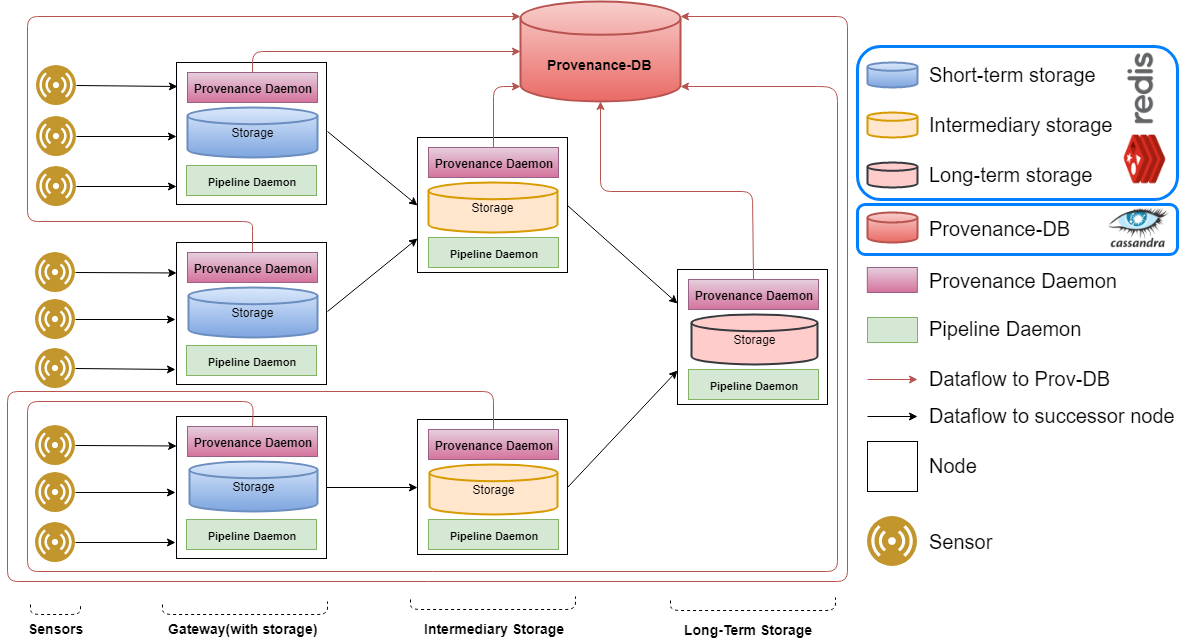
\includegraphics[width=\linewidth]{figures/provenance_system.png}\\
\caption{Provenance System}
\label{provenance_system}
\end{figure}

TODO
